\level{2}{Processo di validazione}
Il processo di validazione serve per determinare se il prodotto finale è conforme a quanto è stato pianificato. Si procederà dapprima ad una validazione interna da parte dei componenti del team e poi sarà il proponente a rivalidare il prodotto, per garantire l’indipendenza del processo.\\
L’attività di validazione consiste nel condurre i test per poi analizzare i risultati e assicurarsi che il prodotto rispecchi le indicazioni per cui è stato sviluppato. Si andrà inoltre a verificare che il prodotto sia abile nell’isolare e minimizzare gli effetti degli errori.\\
Per le norme sulla sintassi dei test si rimanda alla sezione \nameref{sec:test1} del presente documento.

\level{3}{Norme}
\level{4}{Responsabilità}
Di seguito si elencano le rispettive responsabilità per la validazione del prodotto:
\begin{itemize}
	\item il \insrole{Verificatore} ha il compito di eseguire con attenzione i test avendo cura di tracciarne i risultati che andranno poi valutati;
	\item il \insrole{Responsabile di Progetto} revisiona i risultati dei test e decide se accettarli o ripeterli con richiesta di correzione. Ha inoltre l’onere di informare il committente dell’esecuzione e risultato dei test, fornendo indicazioni sulla possibilità di eseguirli in modo indipendente.
\end{itemize}
 

\level{3}{Procedure}
\level{4}{Validazione}
I test verranno dapprima eseguiti manualmente uno per uno dai \insrole{Verificatori}, che ne tracceranno il risultato. Al termine dell’esecuzione dei test il \insrole{Responsabile di Progetto} analizzerà i risultati e deciderà se accettarli, chiedere una ripetizione di alcuni o tutti i test eventualmente con verificatori diversi. Una volta accettati, i risultati verranno consegnati al proponente dal \insrole{Responsabile di Progetto}, che lo informerà sulle modalità di esecuzione indipendente della validazione.

\begin{figure}[H]
	\centering
	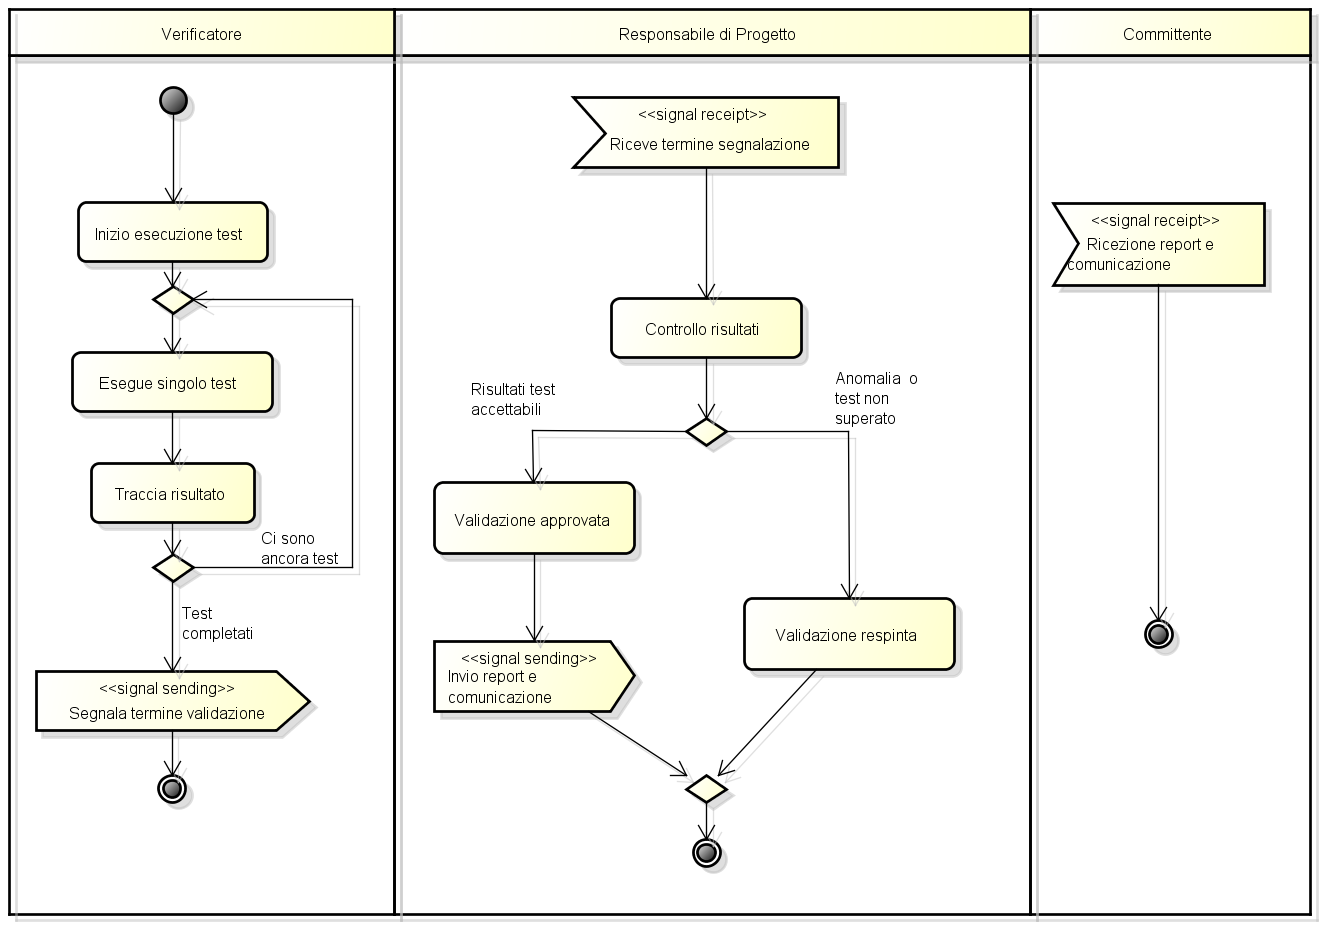
\includegraphics[scale=\textwidth]{Pics/Validazione.png}
	\caption{Procedura di validazione}
\end{figure}
